\documentclass[review]{elsarticle}
\usepackage[utf8]{vietnam}
\setlength{\parskip}{10pt}
%\usepackage[pdftex]{graphicx}
%\usepackage[font=footnotesize]{caption}

\usepackage{mwe}    % loads »blindtext« and »graphicx«
\usepackage{subfig}
\usepackage{float}

\usepackage{mathtools}

\usepackage{lineno,hyperref}
\modulolinenumbers[5]

\journal{Journal of \LaTeX\ Templates}

%%%%%%%%%%%%%%%%%%%%%%%
%% Elsevier bibliography styles
%%%%%%%%%%%%%%%%%%%%%%%
%% To change the style, put a % in front of the second line of the current style and
%% remove the % from the second line of the style you would like to use.
%%%%%%%%%%%%%%%%%%%%%%%

%% Numbered
%\bibliographystyle{model1-num-names}

%% Numbered without titles
%\bibliographystyle{model1a-num-names}

%% Harvard
%\bibliographystyle{model2-names.bst}\biboptions{authoryear}

%% Vancouver numbered
%\usepackage{numcompress}\bibliographystyle{model3-num-names}

%% Vancouver name/year
%\usepackage{numcompress}\bibliographystyle{model4-names}\biboptions{authoryear}

%% APA style
%\bibliographystyle{model5-names}\biboptions{authoryear}

%% AMA style
%\usepackage{numcompress}\bibliographystyle{model6-num-names}

%% `Elsevier LaTeX' style
\bibliographystyle{elsarticle-num}
%%%%%%%%%%%%%%%%%%%%%%%

\begin{document}

\begin{frontmatter}

\title{Pseudo-3D Trajectories: An Effective Approach for Motion Representation in Depth Data}

%% Group authors per affiliation:
\author{Chien-Quang LE}
\address{The Graduate University for Advanced Studies}

%% or include affiliations in footnotes:
\author{Duy-Dinh LE}
\address{National Institute of Informatics}

\author{Shin'ichi Satoh}
\address{National Institute of Informatics}


\begin{abstract}
Leveraging the motion information of trajectories shows the effectiveness to the human action recognition in 2D video. However, the issue is that this approach direction is effective or not when represents motions in 3D video is not still answered. In this paper, we will deal with this issue by conducting experiments based on 2D trajectory features to present motion information from one 3D video representation. Beside, in order to ensure including depth information, we propose a method based on compensating motion information from other representations. Evaluated on the benchmark datasets, our method significantly outperforms the 3D SoA methods.
\end{abstract}

\begin{keyword}
\texttt{Trajectory}\sep action recognition\sep depth\sep feature representation
%\MSC[2010] 00-01\sep  99-00
\end{keyword}

\end{frontmatter}

\linenumbers

\section{Introduction}

\paragraph{Background and Challenges} Gần đây, với sự phát triển của RGB-D camera như Kinect, depth data đã mở ra nhiều hướng nghiên cứu tiềm năng cho bài toán Human Action Recognition. So sánh với intensity images thông thường, depth maps hỗ trợ nhiều advantages hơn. Ví dụ, depth maps cung cấp các thông tin về shape rõ ràng hơn so với intensity images. Hơn thế nữa, depth data ít bị ảnh hưởng bởi những thay đổi của ánh sáng. Tuy nhiên, các phương pháp dựa trên intensity liệu có hiệu quả trên depth data hay không vẫn chưa được quan tâm nhiều.

\paragraph{Existing approaches and drawbacks} Trong bài toán action recognition, để adapt các phương pháp dựa trên intensity cho depth data có 2 yếu tố chính. Thứ nhất, để capture motion information hiệu quả việc chọn lựa a robust feature representation là rất quan trọng. Thứ hai, để đảm bảo motion là đầy đủ thông tin trong depth video, việc bổ sung thông tin depth vào feature representation là yêu cầu không thể thiếu. Tuy nhiên, các phương pháp được đề xuất gần đây vẫn chưa hội tụ đủ 2 yếu tố này. Một số phương pháp như [DMM-HOG, DSTIP-DCSF] xem xét depth value như là intensity value và adapt các intensity-based techniques. Mặc dù, chúng có thể đạt được những kết quả hợp lý, nhưng tất cả chúng đều phải đối mặt với nhiều hạn chế. [DMM-HOG] có thể tận dụng thông tin depth từ các phép chiếu của depth maps. Nhưng its feature representation dựa trên global motion như HOG sẽ dễ gây nhầm lẫn bởi những similar postures. [DSTIP-DCSF] có thể đảm bảo depth information trong việc tính toán features. Nhưng cách tiếp cận này không đảm bảo được sự tin cậy khi extract các local points, do bởi textureless data and depth noise. Ngoài hướng tiếp cận trên, các phương pháp như [LOP, HON4D] chỉ tập trung khai thác depth information nên không tận dụng được sức mạnh của các intensity-based features. Do đó, hướng nghiên cứu của chúng tôi là propose một phương pháp có thể đáp ứng đầy đủ cả 2 yếu tố nêu trên.

\paragraph{Proposal, Idea and Steps}Trong bài báo này, chúng tôi sử dụng một feature representation dựa trên dense trajectories của [Heng Wang], do bởi hiệu quả của cách tiếp cận này trong nhiều bài toán, including activity recognition and multimedia event detection. Các trajectories thu được bằng cách tracking các sampled points densely sử dụng optical flow fields. Sau khi extract trajectories, các trajectory-aligned descriptors sẽ được adopted. Sau đó, features tính toán được từ các descriptors này sẽ được sử dụng cho việc biểu diễn motion information trong video.

Tuy nhiên, việc thiếu sót depth information trong feature representation có thể gây ra các trường hợp bị confused, như được chỉ ra trong Figure \ref{subfig-1:FrontView}. Do đó, để đảm bảo việc không bỏ sót thông tin depth, ý tưởng cơ bản là combine thông tin chuyển động từ nhiều góc nhìn khác nhau. Các biểu diễn từ nhiều góc nhìn có thể đạt được bằng cách chiếu depth maps lên trên các mặt phẳng tương ứng. Việc chiếu này dễ dàng thực hiện được bởi những thuận lợi mà depth data mang lại.

\begin{figure}[H]
	\begin{center}
		\subfloat[From front view\label{subfig-1:FrontView}]{ %
			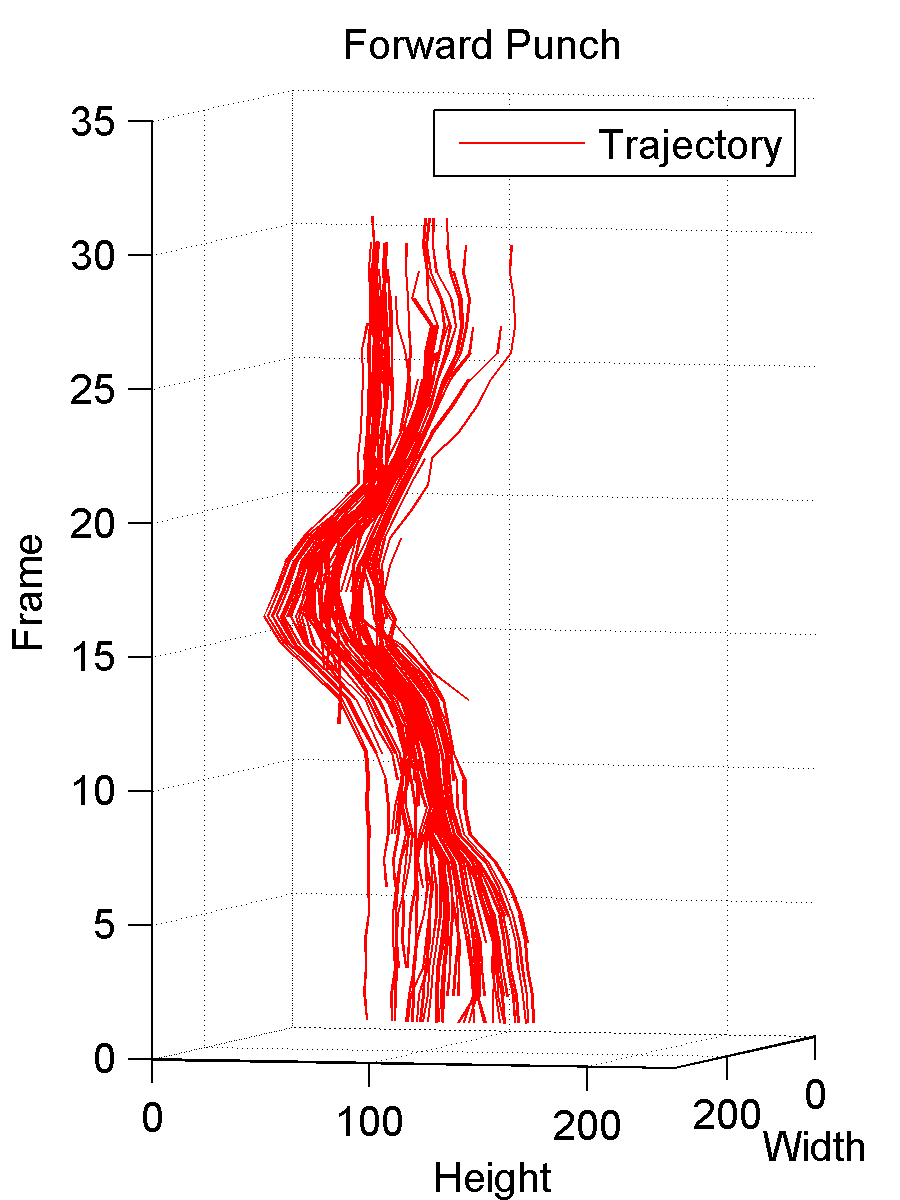
\includegraphics[scale=0.5]{ForwardPunch_FRONT.png}
			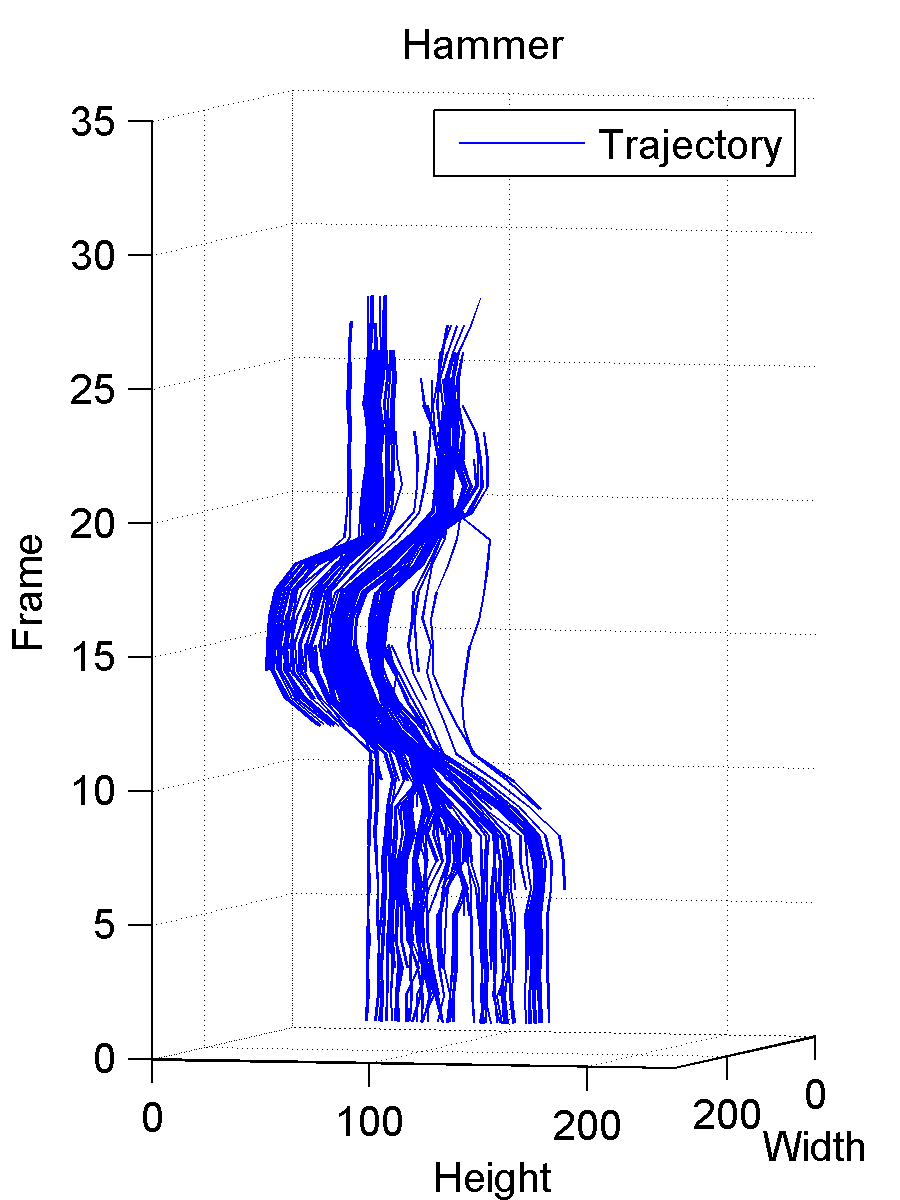
\includegraphics[scale=0.5]{Hammer_FRONT.png}
		}
	\end{center}
	\begin{center}
		\subfloat[From side view\label{subfig-2:SideView}]{ %
			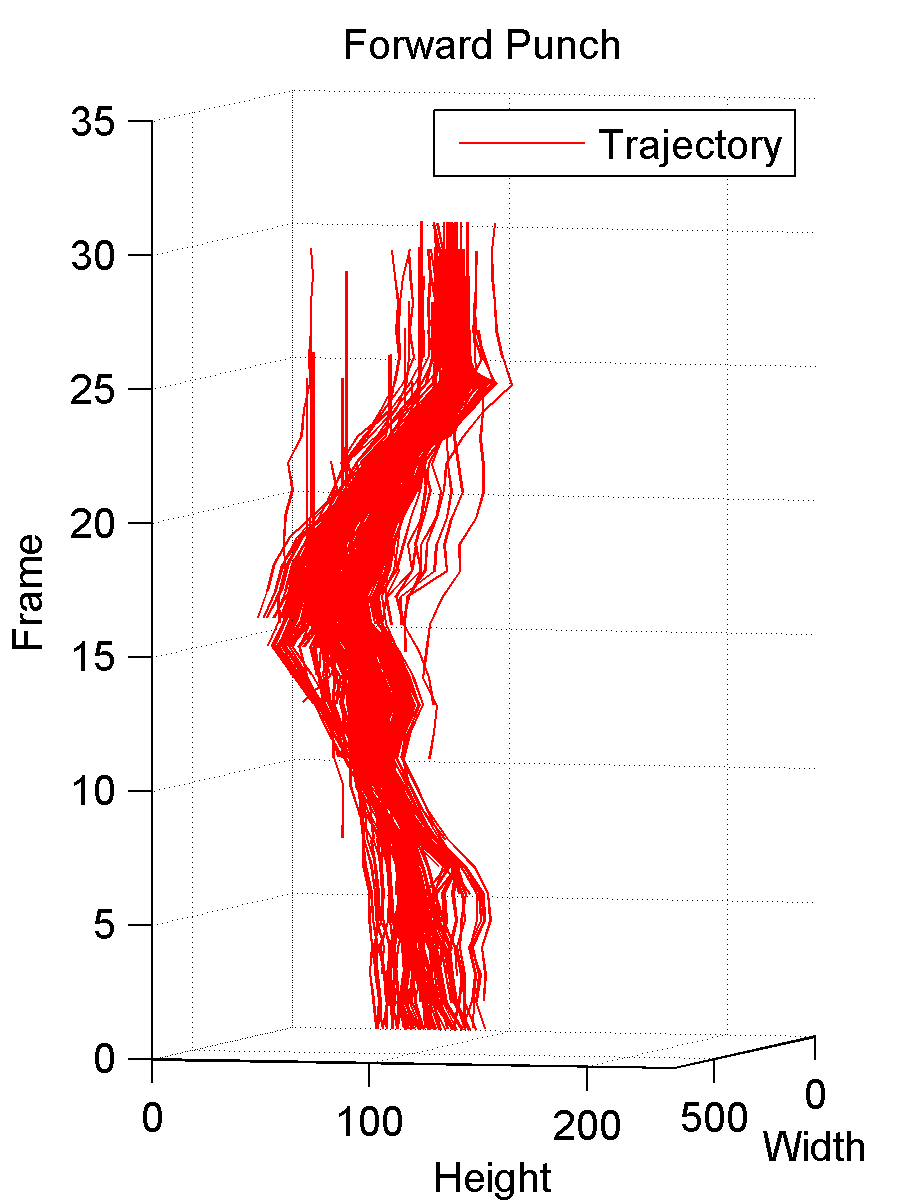
\includegraphics[scale=0.5]{ForwardPunch_SIDE.png}
			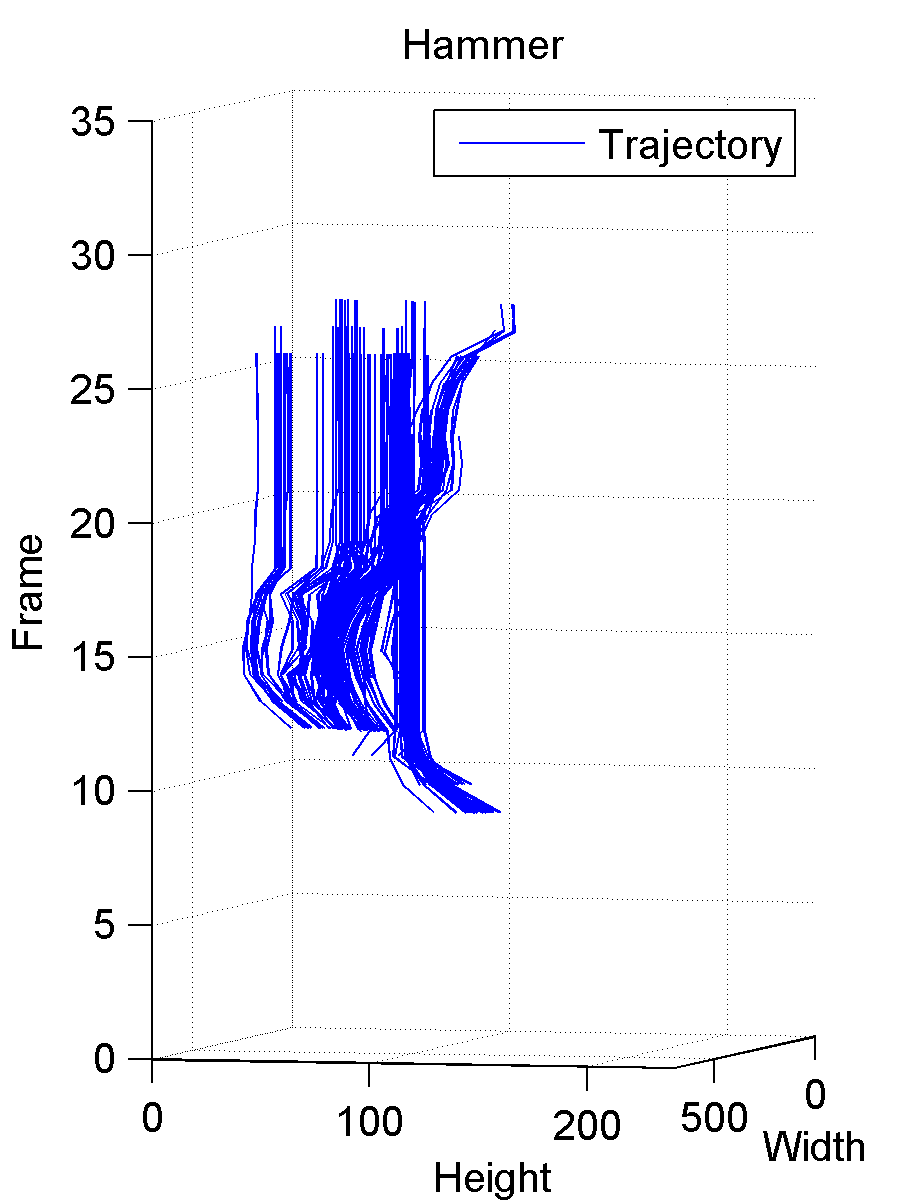
\includegraphics[scale=0.5]{Hammer_SIDE.png}
		}
	\end{center}
	\begin{center}
		\subfloat[From top view\label{subfig-3:TopView}]{ %
			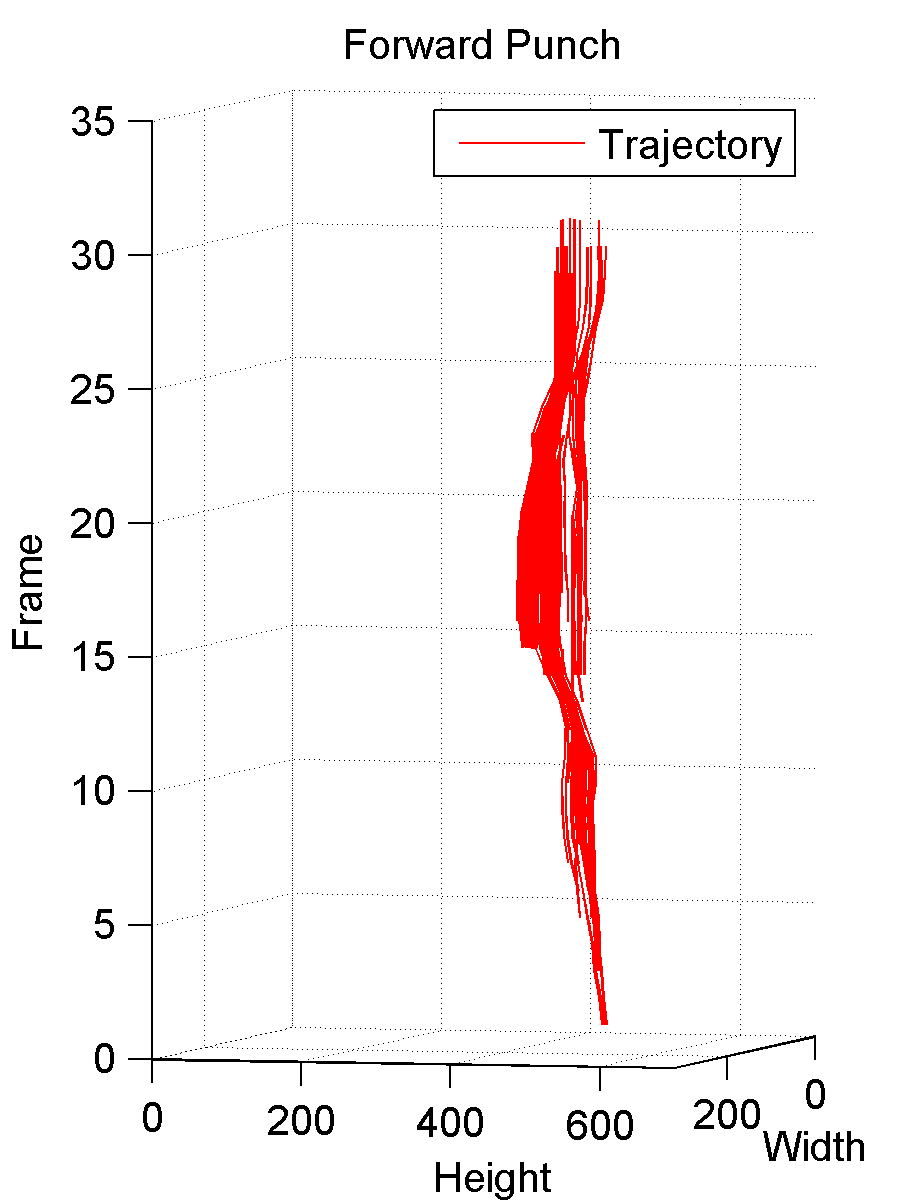
\includegraphics[scale=0.5]{ForwardPunch_TOP.png}
			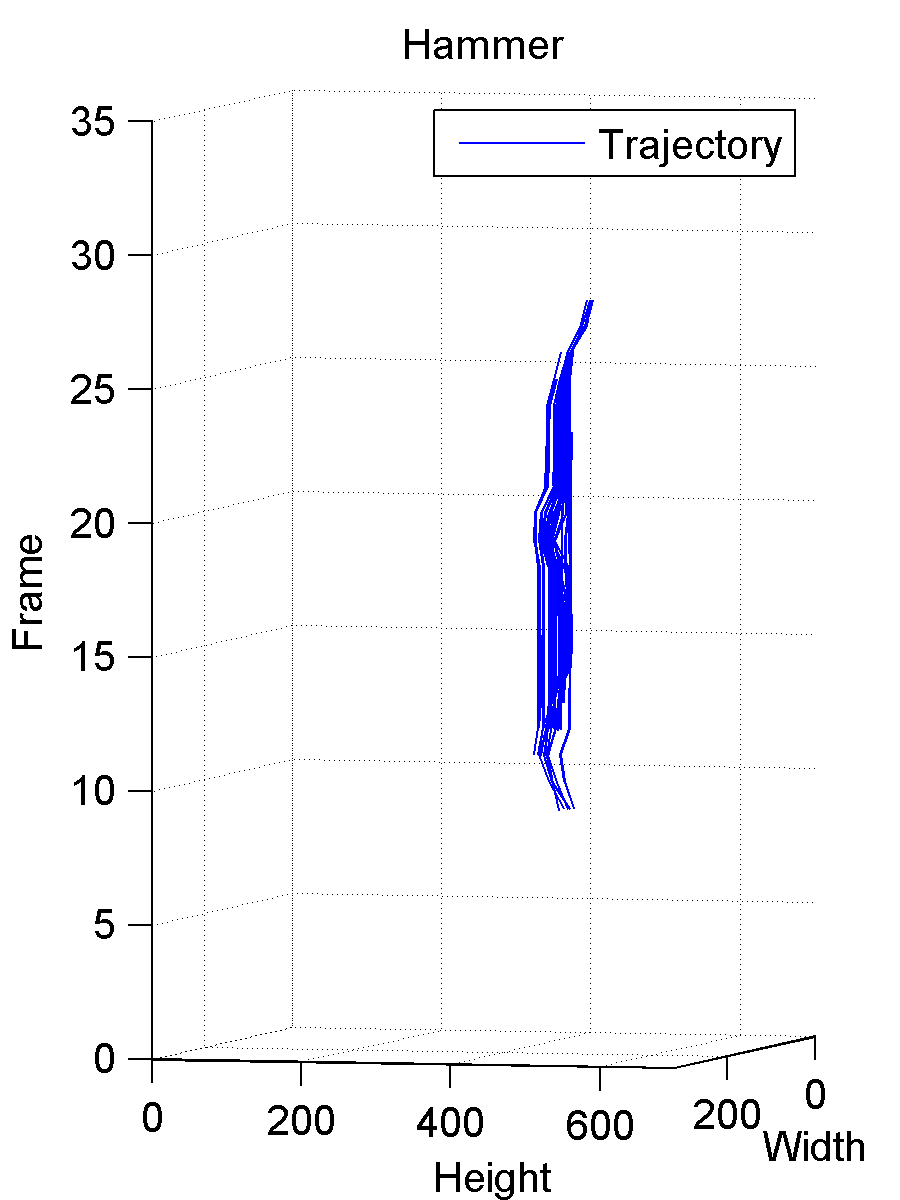
\includegraphics[scale=0.5]{Hammer_TOP.png}
		}
	\end{center}
	\caption{\label{fig:Illustration}Minh họa sự tương tự giữa phần lớn các Trajectories của 2 actions: Forward Punch \& Hammer.}
\end{figure}

\paragraph{Experiments and Results}Chúng tôi tiến hành các experiments trên challenging benchmark datasets, các kết quả thí nghiệm chỉ ra rằng phương pháp của chúng tôi đánh bại the SoA methods trên depth data. Các kết quả này đã cho thấy những contributions của our method: (1) We propose an adaptive method for 3D video representation by using 2D features. (2) We thực hiện comprehensive experiments on the state-of-the-art MSR Action 3D dataset and show that our method is the best when compared with the state-of-the-art 3D methods.

\paragraph{Paper structure}After a brief review of the related work in Section 2, the proposed method is described in Section 3. Section 4 presents the experimental results and their concerned discussions. The summaries of our work are given in Section 5.

\section{Related Works}

Tìm hiểu các thành phần của một hệ thống HAR hiện là một trong những hướng nghiên cứu quan trọng của CV.
Feature representation là 1 trong số các thành phần thu hút được sự chú ý của cộng đồng nghiên cứu.

\paragraph{Works trích chọn features từ depth data}
- Hướng xem depth value như intensity value.
- Hướng sử dụng real depth value và skeleton information.

\paragraph{Điểm khác biệt của phương pháp hiện tại với các phương pháp trước}
- Hướng sử dụng 2d trajectories cho 3d data.

\paragraph{Works in combining many types of features and sự khác biệt với our work}
- Works gần đây sử dụng early fusion sheme.
- Our method sử dụng late fusion sheme.

\section{Proposed Method}
This paper presents a effective depth video representation by adapting intensity trajectories-based motion features. First, chúng tôi sẽ cung cấp một brief review of the dense trajectories-based feature proposed by Heng Wang et al. [DenseTraj2011]. Những phần liên quan như: dense sampling, tracking and feature descriptors is referred to. Our trajectories-based approach for depth data is mentioned at the end of this section.

\subsection{Dense trajectories}
% - Giới thiệu khái quát về dense trajectories
In order to obtain trajectories, there are two important steps: sampling and tracking. [DenseTraj2011] propose sampling on a dense grid with a step size of 5 pixels. The sampling is performed at multiple scales with a factor of $1/\sqrt{2}$. Then, tracking is the next step to form trajectories. At each scale, in frame \textit{t}, each point \textit{$P_t = (x_t, y_t)$} is tracked to point \textit{$P_{t+1} = (x_{t+1}, y_{t+1})$} in next frame \textit{t+1} by:
\begin{equation}
	\textit{$P_{t+1} = (x_{t+1}, y_{t+1}) = (x_t, y_t) + (M*\omega)|_{(\bar{x}_t,\bar{y}_t)} $},
\end{equation}
where \textit{$\omega = (u_t, v_t)$} denotes the dense optical flow field, \textit{M} is the kernel of median filtering, and \textit{$(\bar{x}_t,\bar{y}_t)$} is the rounded position of \textit{$P_t$}. The algorithm of [Farneback, G - Two-Frame Estimation...] is adopted to compute the dense optical flow. And to avoid a drifting problem, a suitable value of trajectory length is set to 15 frames. Beside, trajectories with sudden changes are removed.

After extracting trajectories, two kinds of descriptors: a trajectory shape descriptor and a trajectory-aligned descriptor can be adopted.

\paragraph{Trajectory Shape Descriptor}This descriptor describes the shape of a trajectory in the simplest way. Given a trajectory of length L, its shape is concatenated by a sequence of displacement vectors \textit{$S = (\Delta P_t, ..., \Delta P_{t+L-1})$}, where \textit{$\Delta P_t = P_{t+1} - P_t = (x_{t+1} - x_t, y_{t+1} - y_t)$}. In order to make the descriptor invariant to scale changes, the final result is then achieved by normalizing the shape vector by the overall magnitude of the displacement vectors:

\begin{equation}
	\textit{$\bar{S} = \frac{(\Delta P_t, ..., \Delta P_{t+L-1})}{\sum_{k=t}^{t+L-1}\|\Delta P_k\|}$},
\end{equation}

\paragraph{Trajectory-aligned Descriptor}The descriptors are much more complex than the trajectory shape descriptor. They are computed within a space-time volume ($N \times N$ spatial pixels and $L$ temporal frames) around the trajectory. This volume is divided into a 3D grid (spatially $n_\sigma \times n_\sigma$ grid and temporally $n_\tau$ segments). The default settings of these parameters are $N$ = 32 pixels, $L$ = 15 frames, $n_\sigma$ = 2, and $n_\tau$ = 3.

In order to capture the local motion and appearance around a trajectory, three kinds of descriptors have been employed: the Histogram of Oriented Gradient (HOG) [Dalal et al. Histogram of Oriented Gradients], the Histogram of Optical Flow (HOF) [Laptev et al. Learning Realistic 2008], and the Motion Boundary Histogram (MBH) [Dalal et al. Human detection using oriented histograms of flow 2006]. For HOG, orientation information is quantized into 8-bin histogram. HOF is 9-bin histogram. Since the feature of a trajectory is calculated and concatenated from sub-volumes of a 3D volume, the final representation has 96 dimensions for HOG and 108 dimensions for HOF. MBH descriptor computes derivatives on both horizontal and vertical components of optical flow $I_\omega = (I_x. I_y)$. Similar to HOG descriptor, the orientation information is quantized into 8-bin histogram. Since the motion information is combined along two directions, the final representation is $96 \times 2 = 192$-bin histogram. By presenting gradient of optical flow, MBH descriptor is able to suppress global motion information and only keep local relative changes in pixels.

According to the authors [Laptev et al. 2008 Learning Realistic human ...], [Wang.H et al. 2008 Evaluation of local Spatio-temporal features...], [Liu.J et al. 2009 Recognizing realistic actions from video...], [Wang.H et al. 2011 Action Recognition by dense trajectories...], all the three descriptors have shown the effectiveness for action recognition. The experimental settings for these descriptors are based on an empirical study showed in [Wang.H et al. 2011 Action Recognition by dense trajectories...]. We also conduct our experiment on all the three descriptors when compared to the depth-based state-of-the-art methods.

\subsection{Pseudo-3D trajectory-based Approach for Motion Feature in Depth Data}

Our proposed trajectory-based approach for human action recognition in depth data is as follow. At first, intensity representations are formed from the sequence of depth maps, as illustrated in Figure 2. In particular, we choose number of the representations of 3. Number 3 represents 3 view directions: front, side, and top in 3D space. Forming the representations is necessary due to dimensional gap when we adapt 2D techniques for 3D data. After that, the dense trajectories are extracted from the intensity representations. And the feature descriptors are also computed in this step. At the next step, with each intensity representation, corresponding feature representation is quantized from raw trajectory features by apply a "bag-of-words" model. A "late fusion" scheme is used to generate the final feature representation for action in the sequence of depth maps (Fig. 3).

- Hình 2 - Illustration of proposed method - Depth maps -> 3 projections -> dense trajectories

- Hình 3 - Framework overview for our system - Depth data -> 3 feature extraction -> 3 BoW model -> 3 histogramintersection-SVM -> concatenated-score features -> cai-kernel SVM classifier

In order to generate intensity representations from the sequence of depth maps, we use the approach proposed in [Bag of 3D points]. This technique is also used in [DMM-HOG]. Basically, this method projects depth maps onto three orthogonal planes in Casterian space to obtain corresponding intensity representations. However, motion representation for human action in the previous approaches is accumulated from global motion information. Therefore, these approaches must deal with the challenges from human segmentation problem in more complicated datasets. In contrast to the previous ones, we pay attention to capture local motion information for representing human actions. With the approach, we do not care the challenges for segmenting human body. To effectively use local motion information, we leverage the effectiveness of trajectory-based representation. In practice, we adopt the dense trajectory-based approach proposed in [DenseTraj-2011, Heng Wang]. Thus, motion information in depth data can be reproduced by complementary motion information in different intensity representations.

Our proposed trajectory-based approach is compared with the state-of-the-art methods in human action recognition using depth data. Actually, our approach does not care skeleton extraction, which is used as an important factor in some works, such as [LOP], [3D-EigenJoints]. In fact, extracting skeleton exactly is still an unsolved problem, due to the challenges, such as: cluttered background, hardware quality, camera motion, ... Figure 4 illustrates an example case when extract skeleton information.

- Hình 4 - An example for skeleton extraction error.

\section{Experimental Settings}

\subsection{Dataset}
We test our method on MSR Action 3D dataset. This dataset contains 20 actions, as showed in Table \ref{lbl:20actions}. Actions are performed by ten subjects for two or three times in the context of game console interaction. In total, there are 567 sequences of depth maps. The depth maps are shot at frame rate of 15 fps. The size of the depth map is $640 \times 480$, we resize into $320 \times 240$ to ensure processing efficiency.

\begin{table}[H]
	\begin{center}
		% Table generated by Excel2LaTeX from sheet 'Sheet3'
		\begin{tabular}{c|c|c|c}
		
		{\bf Action Name} & {\bf Action Name} & {\bf Action Name} & {\bf Action Name} \\
		\hline
		 high arm wave &     high throw &  two hand wave &        jogging \\
		
		horizontal arm wave &         draw x &    side-boxing &   tennis swing \\
		
		        hammer &      draw tick &           bend &   tennis serve \\
		
		    hand catch &    draw circle &   forward kick &     golf swing \\
		
		 forward punch &      hand clap &      side kick & pick up \& throw \\
		
		\end{tabular}
	\end{center}
	\caption{\label{lbl:20actions}20 actions in MSR Action 3D dataset}
\end{table}

In order to conduct a fair comparison, we use the same experimental settings as [Bag of 3D points, EigenJoints, DMM-HOG, LOP, DSTIP-DCSF, HON4D]. In the settings, the dataset is divided into three action subsets. Each subset has 8 actions (Table \ref{lbl:3ActionSubsets}). The two subsets AS1 and AS2 present that grouped actions have similar movements. The subset AS3 groups complex actions together. For instance, action $hammer$ seems to be confused with action $forward punch$ in AS1 or similar movements between action $hand catch$ and action $side\ boxing$ in AS2. As for each subset, we select half of the subjects as training and the rest as testing (Cross Subject test).

\begin{table}[H]
	\begin{center}
		% Table generated by Excel2LaTeX from sheet 'Sheet3'
		\begin{tabular}{c|c|c}
		
		{\bf Action Subset 1} & {\bf Action Subset 2} & {\bf Action Subset 3} \\
		{\bf(AS1)} & {\bf(AS2)} & {\bf(AS3)} \\
		\hline
		horizontal arm wave &  high arm wave &     high throw \\
		
		        hammer &     hand catch &   forward kick \\
		
		 forward punch &         draw x &      side kick \\
		
		    high throw &      draw tick &        jogging \\
		
		     hand clap &    draw circle &   tennis swing \\
		
		          bend &  two hand wave &   tennis serve \\
		
		  tennis serve &    side-boxing &     golf swing \\
		
		pick up \& throw &   forward kick & pick up \& throw \\
		
		\end{tabular}
	\end{center}
	\caption{\label{lbl:3ActionSubsets}The three action subsets used in the experiments}
\end{table}

\subsection{Evaluation Method}
- Sử dụng thư viện online để extract DT
- Mô tả các settings trong framework: Number of codewords, assignment method, BoW model, SVM ở 2 pha phân lớp
- Thư viện libsvm
- Đánh giá dựa trên accuracy

\section{Experimental Results}

\subsection{Recognize actions from single-view}
- Mô tả thí nghiệm trên 1 view
- Table - Kết quả trên front view
- Nhận xét các trường hợp bị confused, lý giải dựa trên trajectory shape
- Figure - Ví dụ về các trường hợp bị confused

\subsection{Fuse motion information from all views}
 Our method beats all the state-of-the-art methods based on silhouette features [Bag of 3D points, DMM-HOG], skeletal joint features [EigenJoints, LOP], local occupancy patterns[STOP, ROP], normal orientation features [HON4D] and cuboid similarity features [DSTIP\&DCSF].
 
- Mô tả thí nghiệm trên 3 view
- Table - So sánh với SoA
- Đánh giá lại các trường hợp bị confused
- Figure - Ví dụ về trajectories trên các views khác

\subsection{The impact of our method on descriptors}
- Mô tả thí nghiệm trên 3 descriptors: HOG, HOF, MBH
- Nhận xét trước khi fusion
- Nhận xét sau khi khi fusion:
    + Compensate information
    + Keep salient information

\section{Conclusions}

\paragraph{Tóm tắt our work}

\paragraph{Đề xuất cho future work}



\section*{References}

\paragraph{Cách cite ref}Here are two sample references: \cite{Feynman1963118,Dirac1953888}.

\bibliography{mybibfile}

\end{document}